\section{Geometry, Simulation, and Dataset}\label{sec:dataset}

\subsection{Receiver geometry}
Our four-receiver array covers only the vertical side walls---the $\pm x$ and
$\pm z$ faces---with no coverage on the $\pm y$ top/floor faces, which makes $y$
the hardest axis. An anti-symmetric height placement (P1, P3 at $y={+}6.8$\,cm;
P2, P4 at $y={-}7.3$\,cm) breaks the $y\!\to\!-y$ mirror symmetry enough to
recover $y$ in simulation. The phantom is a benchtop tank with internal
dimensions $273\,(x)\times278\,(y)\times380\,(z)$\,mm, where $y$ is the
\emph{vertical} (height) axis. Only the separate mirror-symmetric ablation array
in Section~\ref{sec:res-modality} is unobservable by construction. Geometry
exploration is closed for this study; the asymmetry is treated as a fixed
property of a four-receiver rig, not a free parameter.
Figure~\ref{fig:geometry} confirms that the $\pm y$ faces carry no receiver
coverage and that the main array uses anti-symmetric receiver heights.

\begin{figure}[t]
\centering
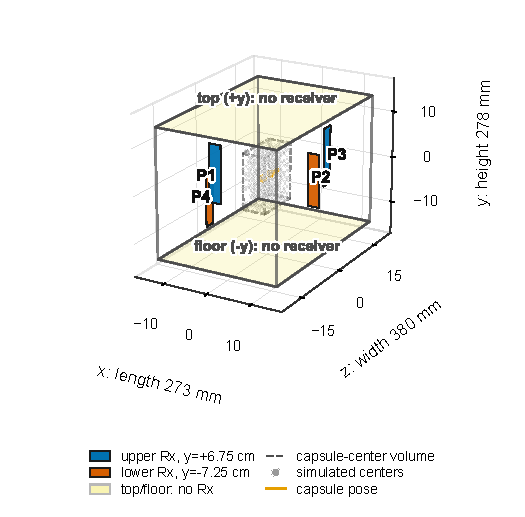
\includegraphics[width=0.94\linewidth]{figures/fig_geometry.pdf}
\caption{Four-receiver side-wall array used by the processed simulation dataset,
drawn with $y$ (height) as the vertical axis. The outer
wireframe is the $273\,(x)\times278\,(y)\times380\,(z)$\,mm tank
envelope; the shaded \emph{top} ($+y$) and \emph{floor} ($-y$) faces carry
\emph{no receiver}, confirming that $y$ has no face coverage. The dashed box
marks the capsule-center sampling volume; the grey cloud shows the $788$
simulated capsule centres. The four receiver patch symbols sit on the vertical
$\pm x/\pm z$ side walls and are placed anti-symmetrically in height (green:
P1/P3 upper, $y={+}6.8$\,cm; orange: P2/P4 lower, $y={-}7.3$\,cm), breaking the
$y\!\to\!-y$ symmetry; contrast the unobservable mirror-symmetric ablation in
Section~\ref{sec:res-modality} (Fig.~\ref{fig:geom-ablation}).
\textbf{Simulation.}}
\label{fig:geometry}
\end{figure}

\subsection{Full-wave simulation}
Channels are computed by full-wave electromagnetic simulation in CST Studio Suite 2025
using a full-wave sweep over \SIrange{380}{430}{MHz}, centred on the legal
MICS/MedRadio band \SIrange{401}{406}{MHz}; the coherent sub-band is
${\sim}$\SIrange{402}{405}{MHz}. The narrow-band production sweep agrees with
the full-band reference to within \SI{0.26}{dB} at \SI{403}{MHz}. These are
full-wave fields, not a parametric path-loss model, so the channel captures
multipath and near-field coupling that bound-based prior art omits
(Section~\ref{sec:related}).

\begin{table}[t]
\centering
\caption{CST reproducibility checklist for the corrected four-receiver simulation data. \textbf{Simulation.}}
\label{tab:cst-repro}
\scriptsize
\setlength{\tabcolsep}{3pt}
\begin{tabular}{@{}p{0.31\linewidth}>{\raggedright\arraybackslash}p{0.63\linewidth}@{}}
\toprule
Item & Repository-grounded value \\
\midrule
Project and units & CST Studio $2025.0$ Microwave Studio; length unit mm \\ % source: wce-cfm/Concepts/CST project design.html:29-39
Body dimensions & $273\times278\times380$\,mm envelope in the paper coordinate convention ($x/y/z$, with $y$ vertical); dense batch metadata records the same extents as $L_{\mathrm{body}}=273$, $W_{\mathrm{body}}=278$, and $H_{\mathrm{body}}=380$ in CST-native parameter names \\ % source: reports/stage2_y_observability/dense_gen/batches/batch_*.npz:param_names,param_values; verified same tuple in 66 batch files
Receiver locations & Processed dataset metadata uses four effective receiver centres: P1/P3 at $y={+}67.5$\,mm, P2/P4 at $y={-}72.5$\,mm; side-wall offsets are $z={\mp}190.835$\,mm for P1/P2 and $x={\pm}137.335$\,mm for P3/P4. Figure~\ref{fig:geometry} is a schematic reconstruction, not a direct CST CAD export \\ % source: scripts/data/build_dense_raw_rssi4.py:30-38; scripts/data/build_dense_rich_features.py:29-31; data/raw_rich_dense_v4_combined.pkl:sensor_positions
Materials & Bio Tissue/Muscle body phantom, Bio Tissue/Skin outer layer, PVC body-wall layer, copper conductors, polyimide capsule substrate \\ % source: wce-cfm/Concepts/CST project design.html:173-207
Ports & Four external $50\,\Omega$ S-parameter receiver ports on the $-z$, $+z$, $+x$, and $-x$ faces; capsule antenna port $6$ on \texttt{Antenn\_in}/\texttt{Inner\_antenna} \\ % source: wce-cfm/Concepts/CST project design.html:74-123
Solver and boundaries & Frequency Domain (Tetrahedral); all six boundaries expanded open, with no symmetry planes \\ % source: wce-cfm/Concepts/CST project design.html:42-52; reports/stage2_y_observability/new_cst_static_2026-05-19/extracted/Model__3D__ModelHistory.json:52-62
	Mesh settings & Tetrahedral mesh entries with volume and surface gradation $1.5$ and energy adaption are present in the replayed ModelHistory \\ % source: reports/stage2_y_observability/new_cst_static_2026-05-19/extracted/Model__3D__ModelHistory.json:63-94; reports/stage2_y_observability/dense_gen/v4fix_check/proj file listing
	Frequency sweep & Dense narrow-band S-parameter tensor over $380$--$430$\,MHz with $1001$ frequency points \\ % source: reports/stage2_y_observability/point_accuracy_validation_2026-05-28.md:11-12; scripts/data/build_dense_rich_features.py:4-6
Generated artifacts & S-parameter batch tensors and a combined 180-D rich-feature dataset used for the $N=3935$ analysis \\ % source: scripts/data/build_dense_rich_features.py:36-39; reports/stage2_y_observability/rich_unified_benchmark.md:3-6
\bottomrule
\end{tabular}
\end{table}

\subsection{Dataset and feature representation}
Each configuration is reduced to a \SI{180}{}-dimensional ``rich'' feature vector
composed of five blocks: a 4-D received signal strength indicator (RSSI) block,
44-D multi-frequency magnitude, 44-D phase cosine, 44-D phase sine, and 44-D
return loss. The combined dataset contains $N=3935$ configurations spanning
$788$ unique capsule positions, with five orientation poses per position
(identity, $z{+}90^\circ$, $y{+}90^\circ$, $y{+}180^\circ$, $x{+}90^\circ$).
Two documented coverage gaps exist (a 15-configuration setup gap in one batch,
and a final batch of 50 by design) and are accounted for in the analysis.

\paragraph*{Combined set vs.\ initial-stage subset ($N=1980$)}
The dense data were generated in two stages. We refer to the full set
($N=3935$, all $788$ positions) as the \emph{combined set}, and to the
initial-stage subset ($N=1980$, the first $396$ positions $\times$ $5$ poses,
generated before the full sweep completed) as the \emph{initial-stage subset}.
The headline point-accuracy and CFM posterior numbers use the combined set. The
initial-stage subset has two uses: the multi-method UQ bake-off
(Table~\ref{tab:uq}) and the deployability ablation (Table~\ref{tab:deploy}),
both under identical pipelines, geometry, and protocol. We tag every result with
the set it uses. The same CFM model therefore reports a \SI{0.354}{cm} point MAE
on the combined set and \SI{0.501}{cm} on the smaller subset, consistent with a
data-size effect (same model, same pipeline).

\begin{table}[t]
\centering
\caption{Construction of the 180-D rich RF feature vector. \textbf{Simulation.}}
\label{tab:rich-features}
\scriptsize
\setlength{\tabcolsep}{3pt}
\begin{tabular}{@{}p{0.23\linewidth}p{0.16\linewidth}p{0.55\linewidth}@{}}
\toprule
Block & Dimension & Definition \\
\midrule
RSSI block & $4$ & Columns $0$--$3$: $|S_{i5}|$ in dB at the bin nearest \SI{400}{MHz}, one capsule-to-receiver value for each of the four receiver ports \\ % source: scripts/data/build_dense_rich_features.py:11-18,55-68; wce-cfm/Concepts/Rich feature set (180-D).html:121-137
Magnitude & $44$ & Columns $4$--$48$: $|S_{i5}|$ in dB at $11$ evenly spaced bins: \begin{tabular}[t]{@{}l@{}}$380,385,390,395,$\\$400,405,410,415,$\\$420,425,430$\,MHz\end{tabular} \\ % source: scripts/data/build_dense_rich_features.py:36-39,55-59,67-80; reports/stage2_y_observability/point_accuracy_validation_2026-05-28.md:11-12
Phase cosine & $44$ & Columns $48$--$92$: $\cos(\arg S_{i5})$ at the same $11$ frequency bins \\ % source: scripts/data/build_dense_rich_features.py:69-80; wce-cfm/Concepts/Rich feature set (180-D).html:145-151
Phase sine & $44$ & Columns $92$--$136$: $\sin(\arg S_{i5})$ at the same $11$ frequency bins \\ % source: scripts/data/build_dense_rich_features.py:69-80; wce-cfm/Concepts/Rich feature set (180-D).html:152-157
Return loss & $44$ & Columns $136$--$180$: $|S_{ii}|$ in dB at the same $11$ frequency bins \\ % source: scripts/data/build_dense_rich_features.py:64-80; wce-cfm/Concepts/Rich feature set (180-D).html:159-165
Conventions & $180$ total & Magnitudes use $20\log_{10}|S|$ with a $-120$\,dB floor; phase is stored as cosine/sine to avoid wrapping; train-fold normalization uses training indices only \\ % source: scripts/data/build_dense_rich_features.py:61-80; scripts/training/baselines/run_cfm_uq_score.py:220-223; reports/stage2_y_observability/point_accuracy_validation_2026-05-28.md:20-24
\bottomrule
\end{tabular}
\end{table}

\subsection{Evaluation protocol}
All methods are evaluated under \textbf{position-grouped 5-fold cross-validation}
(\texttt{GroupKFold} over the $788$ unique positions) with three seeds
($5\times3 = 15$ fold$\cdot$seed evaluations). Grouping by position guarantees
that all poses of a given position fall in the same fold, so no position is ever
split across train and test; this is materially stricter than the random
point-wise splits used by several comparators, and it removes the
position-leakage that inflates random-split scores. Normalization statistics are
fit on the training fold only. To make method comparisons paired, the same test
indices are reused across methods, and significance is assessed by a
position-paired bootstrap over the $788$ unique coordinates.

\paragraph*{Caveat}
The entire dataset is simulation. No measured-phantom or in-vivo data appear
anywhere in this study.
